\emph{Kelahiran suatu pikiran sering menyamai kelahiran seorang anak. 
Ia didahului dengan penderitaan-penderitaan pembawaan kelahirannya.}\cite{tanmalaka}\\ \\Untuk
memastikan kita benar-benar memahami suatu hal, kita harus memahami konteks historis bagaimana hal itu terlahirkan,
konsekuensi dari perkembangannya, dan kontradiksi internal yang mendahului perkembangannya.

\subsection{Kelahirannya}
Menariknya, sejarah SDLC tidak sedalam sejarah perkembangan \emph{software development}. 
Kerangka framework, "SDLC" yang mempertimbangkan struktur tahapan yang terlibat dalam 
pengembangan aplikasi dari studi kelayakan awal hingga penerapannya di lapangan 
dan pemeliharaan, mulai dikenal dengan model waterfall. Deskripsi formal pertama dari model 
waterfall dikutip dalam sebuah artikel tahun 1970 oleh Winston W. Royce.\cite{Shantanu}

Model Waterfall menyediakan model yang terorganisir dan terkendali 
untuk mengelola proyek; model ini berkembang secara linear melalui 
fase-fase yang diskrit, logis, dan dapat dijelaskan, sehingga mudah dipahami dan 
diimplementasikan. Model ini menyediakan pencapaian yang mudah diidentifikasi dalam proses pengembangan. 

SDLC "berasal dari tahun 1960-an, untuk mengembangkan 
sistem bisnis fungsional berskala besar di era konglomerat bisnis berskala besar. 
Aktivitas sistem informasi berkisar pada pemrosesan data yang berat dan rutinitas penghitungan angka.".\cite[see p.86]{geoffrey}

\emph{Structured Systems Analysis and Design Method} (SSADM) dibuat untuk 
Kantor Perdagangan Pemerintah Inggris pada tahun 1980-an. Sejak saat itu, "pendekatan siklus hidup tradisional untuk pengembangan 
sistem semakin digantikan dengan pendekatan dan kerangka kerja alternatif, yang berusaha 
mengatasi beberapa kekurangan yang melekat pada SDLC tradisional"\cite[see p.86]{geoffrey}

\subsection{Konsekuensi Era yang Berbeda}
Agar kita dapat memahami alasan utama dari kekurangan yang melekat pada metodologi SDLC tradisional, 
kita harus menempatkan pengembangan SDLC ke dalam konteks sejarah yang tepat di mana metodologi tersebut muncul. 

Perkembangan SDLC kurang lebih bersamaan dengan perkembangan \emph{Software Engineering} sebagai 
sebuah disiplin ilmu. Dan karena itu, karena \emph{Software Engineering} awal harus tumbuh dari bidang 
lain untuk membentuk dirinya sendiri sebagai disiplin ilmu yang tepat, maka secara alamiah harus 
tumbuh dari bidang lain yang terkait seperti Matematika, Teknik, Fisika, dll.

Upaya awal untuk tumbuh dengan sendirinya ini adalah salah satu alasan mengapa metodologi 
SDLC awal mengikuti jalur linier yang kaku dan ketat untuk model pengembangannya. 
Sebagai warisan dari nenek moyangnya, pada awalnya, sifat asli perangkat lunak belum sepenuhnya disadari. 
Fleksibilitas, kecepatan, kelincahan, dan kekuatan komputasi yang dapat dihasilkannya, bukanlah karakteristik perangkat 
lunak yang dimanfaatkan sepenuhnya oleh para \emph{Software Engineers} dahulu.

Pengembangan software awal sebagian besar terdiri dari proyek-proyek pemerintah yang sangat terspesialisasi, 
dengan proyek-proyek seperti Proyek SAGE, Apollo Guidance Computer, dll.


\subsection{Era Baru}
Ketika fokusnya bergerak ke arah \emph{Customer Centricity}, model Waterfall mulai mendapat kritik karena modelnya yang bertahap 
secara linier, yang tidak memungkinkan adanya fleksibilitas terhadap perubahan pelanggan di tengah-tengah pengembangan software
dan dalam banyak kasus memiliki waktu yang lama, yang mengakibatkan lamanya waktu penyelesaian.

Pengembangan iteratif diciptakan sekitar tahun 1975 sebagai respons terhadap inefisiensi dan masalah yang ditemukan dalam model Waterfall.
Iteratif dan Inkremental sering kali saling melengkapi dan dalam beberapa proyek, keduanya digunakan bersamaan. 
Fondasi dasar metode ini mendukung pengembangan sistem melalui siklus berulang (Iteratif) dan dalam subset yang 
lebih kecil dalam satu contoh (Inkremental), sehingga memungkinkan tim untuk memanfaatkan pembelajaran dari 
fase sebelumnya dan berimprovisasi dalam iterasi saat ini.

Walau model iteratif dan inkremental saling melengkapi dan berada dalam project yang sama,
kedua model itu tetap mempunyai posisi yang berbeda pada suatu project,
Berikut adalah visualisasi perbedaan antara model iteratif dan inkremental :

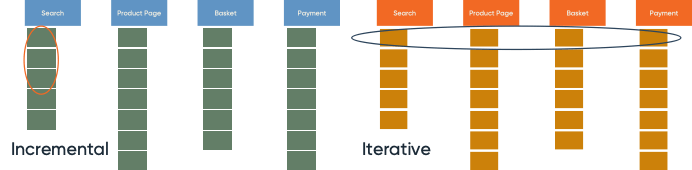
\includegraphics[width=1.1\textwidth, angle=-90]{images/incr-vs-interative.png}

\newpage

Evolusi SDLC terus berlanjut, dengan fokus pada kelincahan dalam upaya untuk mengurangi penyelesaian,
membangun produk yang layak sambil menjaga pelanggan tetap menjadi pusat dari segalanya. 
Hal ini membutuhkan paradigma perubahan yang mengedepankan individu dan interaksi 
daripada proses dan alat, software yang berfungsi daripada dokumen yang komprehensif, 
kolaborasi pelanggan melalui semua fase, dan merespons perubahan daripada mengikuti rencana. 
Kebutuhan saat itu adalah memiliki metode yang lebih fleksibel yang dapat memenuhi kebutuhan tersebut. 
Metode Agile muncul sebagai pengembangan langsung dari metode perangkat lunak dari tahun 1980-an, yaitu

\begin{itemize}
    \item \emph{Joint Application Design} (1986) 
    \item \emph{Rapid Systems Development} (1987)
    \item \emph{Rapid Application Development} (1991).
\end{itemize}
